% libre-compendium
%
% Copyright (C) 2026 Richard Qin
%
% This document is dual-licensed under either:
% - GNU Free Documentation License, Version 1.3 or any later version
%   published by the Free Software Foundation; with no Invariant Sections,
%   no Front-Cover Texts, and no Back-Cover Texts (see COPYING.DOC); or
% - Creative Commons Attribution-ShareAlike 4.0 International License
%   (see LICENSE-CC-BY-SA-4.0).

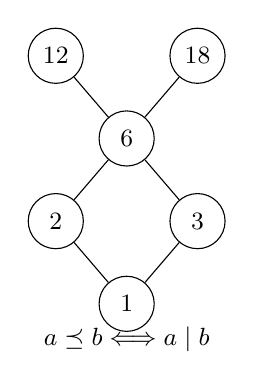
\begin{tikzpicture}[every node/.style={font=\small}]
\tikzstyle{v}=[circle,draw,minimum size=7mm,inner sep=0pt,fill=white]
\node[v] (1) at (0,0) {1};
\node[v] (2) at (-.9,1.05) {2};
\node[v] (3) at (.9,1.05) {3};
\node[v] (6) at (0,2.1) {6};
\node[v] (12) at (-.9,3.15) {12};
\node[v] (18) at (.9,3.15) {18};
\draw (1) -- (2);
\draw (1) -- (3);
\draw (2) -- (6);
\draw (3) -- (6);
\draw (6) -- (12);
\draw (6) -- (18);
\node at (0,-.45) {$a\preceq b \Longleftrightarrow a\mid b$};
\end{tikzpicture}
